%%%%%%%%%%%%%%%%%%%%%%%%%%%%%%%%%%%%%%%%%%%%%%%%%%%%%%%%%%%%%%%%%%%%%%%%%%%%%%%%
%2345678901234567890123456789012345678901234567890123456789012345678901234567890
%        1         2         3         4         5         6         7         8
\documentclass[letterpaper, 10 pt, conference]{ieeeconf}  % Comment this line out
                                                          % if you need a4paper
%\documentclass[a4paper, 10pt, conference]{ieeeconf}      % Use this line for a4

\usepackage{float}
                                                          % paper
% uso paquete bookmark para tener bien los outlines.
\usepackage{bookmark}

% Configuro el idioma.
\usepackage[utf8]{inputenc} % Importante para mantener acentos.
\usepackage[spanish, activeacute]{babel} % Requiere: texlive-lang-spanish. Por primera vez hay que ejecutar: texconfig init> log

% Paquete para poder usar acentos en $$.
\usepackage{mathtools}
%\setmathfont{XITS math}

% Para los diagramas de flujo
\usepackage{tikz}
\usetikzlibrary{shapes.geometric, arrows}

% Elementos del diagrama
\tikzstyle{startstop} = [rectangle, rounded corners, 
minimum width=6em, 
minimum height=2em,
text centered, 
draw=black, 
fill=red!30]

\tikzstyle{io} = [trapezium, 
trapezium stretches=true, % A later addition
trapezium left angle=70, 
trapezium right angle=110, 
minimum width=6em, 
minimum height=2em, text centered, 
draw=black, fill=blue!30]

\tikzstyle{block} = [rectangle, 
minimum width=8em, 
minimum height=3em, 
text centered, 
text width=7.5em, 
draw=black, 
fill=white!30]

\tikzstyle{def} = [rectangle, 
minimum width=14em, 
minimum height=3em, 
text centered, 
text width=12em, 
draw=black, 
fill=purple!30]

\tikzstyle{swap_proccess} = [rectangle, 
minimum width=8em, 
minimum height=2em, 
text centered, 
text width=8em, 
draw=black, 
fill=orange!30]

\tikzstyle{process} = [rectangle, 
minimum width=6em, 
minimum height=2em, 
text centered, 
text width=6em, 
draw=black, 
fill=orange!30]

\tikzstyle{decision} = [diamond, 
minimum width=6em, 
minimum height=6em, 
text centered, 
draw=black, 
fill=green!30]
\tikzstyle{arrow} = [thick,->,>=stealth]

\usepackage{siunitx}

% package to get \url
\usepackage{hyperref}
\hypersetup{
  colorlinks=true,
  linkcolor=magenta,
  filecolor=magenta,
  citecolor=magenta,      
  urlcolor=magenta,
}

% Graficos electrónicos
\usepackage[RPvoltages]{circuitikz}

\IEEEoverridecommandlockouts                              % This command is only
                                                          % needed if you want to
                                                          % use the \thanks command
\overrideIEEEmargins
% See the \addtolength command later in the file to balance the column lengths
% on the last page of the document

\usepackage{graphicx}
\usepackage{graphics}

% styling for matlab/octave code.
\usepackage{matlab-prettifier}
% Configuracion, con esto puede agregar ñ.
\lstset{
  literate={ñ}{{\~n}}1
}

\usepackage{listings}

% The following packages can be found on http:\\www.ctan.org
%\usepackage{graphics} % for pdf, bitmapped graphics files
%\usepackage{epsfig} % for postscript graphics files
%\usepackage{mathptmx} % assumes new font selection scheme installed
%\usepackage{times} % assumes new font selection scheme installed
\usepackage{amsmath} % assumes amsmath package installed
%\usepackage{amssymb}  % assumes amsmath package installed

\title{\LARGE \bf Entregable Trabajo Práctico N° 3}

\author{
  Tom\'as Vidal\\
  {\it Sistemas Operativos y Redes}\\
  {\it Facultad de Ingenier\'ia, UNLP, La Plata, Argentina.}\\
  {\it 30 de Octubre, 2024.}
}                                            % <-this % stops a space


% comienzo

% INTRO


% Figura
\newcommand{\image}[2] {
  \begin{figure}[H]
    \centering
    \includegraphics[width=0.43\textwidth]{./#1.png}
    \caption{#2}
    \label{fig:#1}
  \end{figure}
}

% Codigo
% \begin{lstlisting}[style=Matlab-editor]
% % el código va aca
% dispc("HELLO WORLD");
% \end{lstlisting}

\begin{document}
\maketitle
\thispagestyle{empty}
\pagestyle{empty}

\section{Problema presentado}
Se debe crear un programa que deba ejecutar \textit{dos hilos}: \textbf{hilo A} e \textbf{hilo B}. Ambos deben poder acceder a un \textit{bloque de memoria compartida}, para poder leer y escribir datos en común (\textit{un arreglo de 20 bits}). Ambos procesos deben mantener una cierta sincronía, ya que uno no puede leer mientras el otro escribe y viceversa.

\section{Algorimo implementado}
En la figura \ref{fig:diag_flujo} se muestra el flujo general del programa. El diagrama es \textit{abierto}, en sentido de que hay caminos en paralelo, esto se debe a que el programa tiene un comportamiento concurrente, debido a que se ejecutan múltiples hilos.
\begin{figure*}[tb]
  \centering
  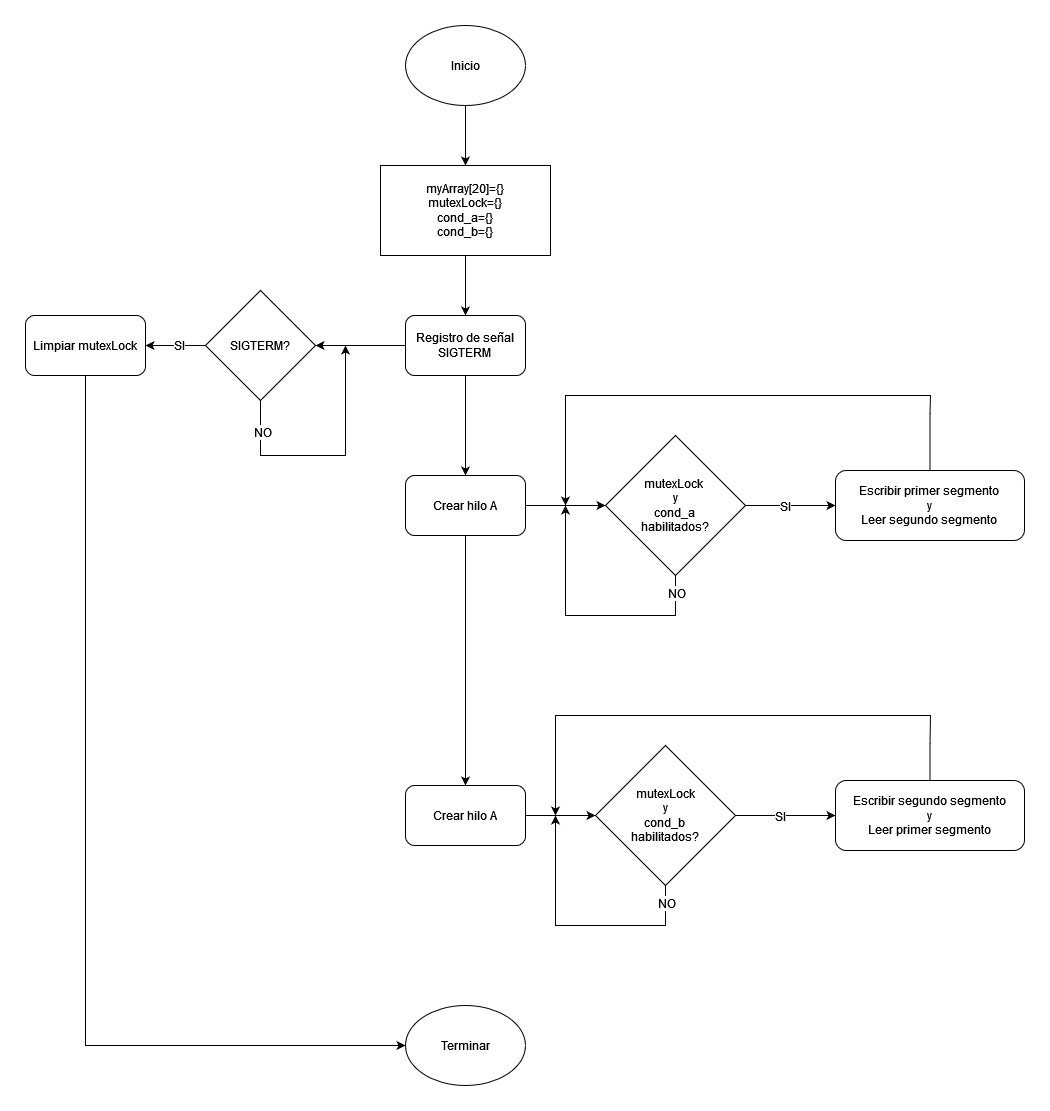
\includegraphics[width=\textwidth]{./tp3diagflujo.png}
  \caption{Diagrama de flujo del algorimo implementado.}
  \label{fig:diag_flujo}
\end{figure*}

\section{Funciones principales}
\begin{itemize}
  \item \textit{handle\_termination:} Manejador que se encarga de liberar los recursos compartidos.
  \item \textit{handle\_thread\_a:} Realiza la escritura y lectura acorde a las especificaciones del \textbf{Hilo A}.
  \item \textit{handle\_thread\_b:} Realiza la escritura y lectura acorde a las especificaciones del \textbf{Hilo B}.
  \item \textit{cypher:} Función de encriptación de datos.
  \item \textit{decypher:} Función de desencriptación de datos.
\end{itemize}

\section{Explicación general del algorimo}
Se registra el manejador para la señal \textbf{SIGTERM}. Luego se crean el \textit{mutex, cond\_a y cond\_b, los hilos A y B}; y se ejecutan los hilos, que quedan en un bucle de ejecución de tiempo indefinido, realizando las escrituras y lecturas acordes a las especificaciones, la sincronización se logra con el mutex y las condiciones compartidas entre los hilos (\textit{cond\_a y cond\_b}). Eventualmente cuando la señal \textbf{SIGTERM} se reciba, se cancelan los bucles de los hilos, y luego de que se terminan las tareas que están realizando finalizan el bucle, se liberan los recursos y finaliza el programa.

Al comienzo se definen los 20 \textbf{int}, que conforman las palabras 'holamundooholaamundo', encriptadas con las especificiones del problema (es decir son \textit{números del 0 al 26}, que representan las letras de la \textbf{a} a la \textbf{z}), posteriormente en la escritura de ambos procesos, se escriben estos datos nuevamente encriptados con la función provista $f(x)$, y cuando se leen se desencriptan con la función $f^{-1}(x)$

\section{Repositorio de Github}
El trabajo se puede encontrar en el siguiente \href{https://github.com/SOyR-2024-Grupo-10/Entregable-practica-3}{repositorio de Github}. \\ 
\textit{Para acceder al mismo se deben tener permisos}

\end{document}
